\documentclass[letterpaper,  %a4paper
               %boxit,
               %titlepage,   % separate title page
               %refpage      % separate references
              ]{jacow-2_3}   %jacow}
%
% CHANGE SEQUENCE OF GRAPHICS EXTENSION TO BE EMBEDDED
% ----------------------------------------------------
% test for XeTeX where the sequence is by default eps-> pdf, jpg, png, pdf, ...
%    and the JACoW template provides JACpic2v3.eps and JACpic2v3.jpg which
%    might generates errors, therefore PNG and JPG first
%
\makeatletter%
	\ifboolexpr{bool{xetex}}
	 {\renewcommand{\Gin@extensions}{.pdf,%
	                    .png,.jpg,.bmp,.pict,.tif,.psd,.mac,.sga,.tga,.gif,%
	                    .eps,.ps,%
	                    }}{}
\makeatother

% CHECK FOR XeTeX/LuaTeX BEFORE DEFINING AN INPUT ENCODING
% --------------------------------------------------------
%   utf8  is default for XeTeX/LuaTeX 
%   utf8  in LaTeX only realizes a small portion of codes
%
\ifboolexpr{bool{xetex} or bool{luatex}} % test for XeTeX/LuaTeX
 {}                                      % input encoding is utf8 by default
 {\usepackage[utf8]{inputenc}}           % switch to utf8

\usepackage[USenglish]{babel}			 

\usepackage[final]{pdfpages}
\usepackage{multirow}
\usepackage{ragged2e}
\usepackage{tikz}
\usetikzlibrary{shapes,arrows,snakes,backgrounds}
\usetikzlibrary{mindmap,trees}
\usetikzlibrary{decorations.pathreplacing}
\usetikzlibrary{plotmarks}
%
% if BibLaTeX is used
%
\ifboolexpr{bool{jacowbiblatex}}%
 {%
  \addbibresource{jacow-test.bib}
  \addbibresource{biblatex-examples.bib}
 }{}
\listfiles

%
% command for typesetting a \section like word
%
\newcommand\SEC[1]{\textbf{\uppercase{#1}}}

%%
%%   Lengths for the spaces in the title
%%   \setlength\titleblockstartskip{..}  %before title, default 3pt
%%   \setlength\titleblockmiddleskip{..} %between title + author, default 1em
%%   \setlength\titleblockendskip{..}    %afterauthor, default 1em

%\copyrightspace %default 1cm. arbitrary size with e.g. \copyrightspace[2cm]

% testing to fill the copyright space
%\usepackage{eso-pic}
%\AddToShipoutPictureFG*{\AtTextLowerLeft{\textcolor{red}{COPYRIGHTSPACE}}}

\begin{document}

\title{Photoinjector Optimization Studies at the AWA}

\author{N. Neveu\thanks{nneveu@anl.gov}\textsuperscript{1}, 
	    L. Spentzouris, Illinois Institute of Technology, Chicago, USA \\
	    J. Larson, J. G. Power, \textsuperscript{1}Argonne National Laboratory}
\maketitle

%
\begin{abstract}
With a variable charge range of 0.1 nC - 100 nC, 
the Argonne Wakefield Accelerator facility (AWA) 
has a unique and dynamic set of operating parameters. 
Adjustment of the optics and occasionally the rf phases is 
required each time the bunch charge is changed. 
Presently, these adjustments are done by the operator during each experiment. 
This is time consuming and inefficient, more so at high charge and for complex experimental set ups.
In an attempt to reduce the amount of time spent adjusting parameters by hand, 
several optimization methods in simulation are being explored. 
This includes using the well-known Genetic Algorithm (NSGA-II),
incorporated into OPAL-T. 
We have also investigated a model-based method and novel
structure based algorithms developed at ANL. 
Ongoing efforts include using these optimization methods to improve operations at the AWA. 
Simulation results will be compared to measured beam parameters at the AWA, 
and one or more optimization methods will be selected for use in guiding operations in the future.
\end{abstract}


\section{AWA Facility}
The AWA Facility houses two rf photoinjectors, both 
operating at \SI{1.3}{GHz}. 
This beam line is capable of low (\SI{0.1}{nC}) and 
high charge (\SI{100}{nC}) operation. The bunch charge is 
routinely adjusted depending on the requirements 
of the experiments downstream of the photoinjector.
Typical operating charges are 1, 4, 10, and \SI{40}{nC}. 
While these are the most
common operating modes, other charges have been requested 
and provided depending on the experiment.
Recent experiments include emittance exchange \cite{eex}, 
structure tests \cite{pets}, thermal emittance measurements \cite{therm}, 
and Two Beam Acceleration (TBA) \cite{tba}. 

\section{Model Based Method}
Last year, we began with the optimization of the front end of 
the high charge photoinjector at the AWA. The charge
of interest was \SI{40}{nC}, and chosen to target the needs 
for upcoming TBA experiments at AWA.
The simulation model included the gun, two solenoids, 
and six accelerating cavities, as shown in Fig.~\ref{beamline}. 
The quadrupoles and bending elements were not included in this work.
We choose ten variables for the optimization parameters: 
laser radius, laser full width half maximum, solenoid strength ($S_2$), 
gun cavity phase, and the six accelerating cavity phases ($\phi_{L_1}-\phi_{L_6}$).
\begin{figure*}%[!tbh]
	\centering
	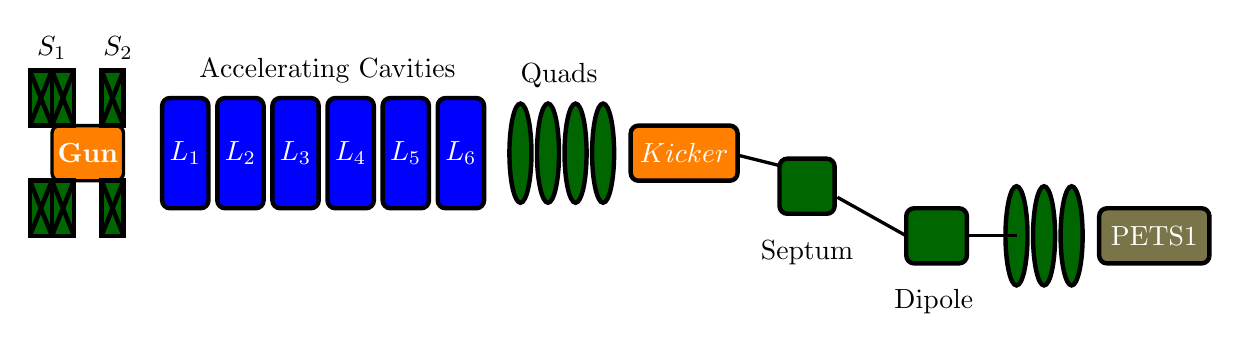
\begin{tikzpicture}[scale=0.7, text=black]
	\def \gunleft {-1.0}
\def \gunright {0.3}
\def \loneright {1.0}
\def \ltworight {2.0}
\def \lthreeright {3.0}
\def \lfourright {4.0}
\def \lfiveright {5.0}
\def \lsixright {6.0}
\def \quadone {7.5}
\def \quadfour{16}

\draw[fill=orange, very thick, rounded corners =0.1cm] (\gunleft,0.5)rectangle (\gunright,1.5) node[pos=.5, white] {\textbf{Gun}} ;

%S1
\node[] at (-1,2.9) {$S_1$};
\draw[ultra thick, fill=black!60!green] (-1.4,-0.5)rectangle  (-1.0,0.5) node[pos=.5, white] {} ;
\draw[black, ultra thick] (-1.4,-0.5) -- (-1.0,0.5);
\draw[black, ultra thick] (-1.4,0.5) -- (-1.0,-0.5);
\draw[ultra thick, fill=black!60!green] (-1.4,1.5)rectangle  (-1.0,2.5) node[pos=.5, white] {} ;
\draw[black, ultra thick] (-1.4,1.5) -- (-1.0,2.5);
\draw[black, ultra thick] (-1.4,2.5) -- (-1.0,1.5);
%S2

\draw[ultra thick, fill=black!60!green] (-1.0,-0.5)rectangle  (-0.6,0.5) node[pos=.5, white] {} ;
\draw[black, ultra thick] (-1.0,-0.5) -- (-0.6,0.5);
\draw[black, ultra thick] (-1.0,0.5) -- (-0.6,-0.5);
\draw[ultra thick, fill=black!60!green] (-1.0,1.5)rectangle  (-0.6,2.5) node[pos=.5, white] {} ;
\draw[black, ultra thick] (-1.0,1.5) -- (-0.6,2.5);
\draw[black, ultra thick] (-1.0,2.5) -- (-0.6,1.5);

%S3
\node[] at (0.2,2.9) {$S_2$};
\draw[ultra thick, fill=black!60!green] (-0.1,-0.5) rectangle  (0.3,0.5) node[pos=.5, white] {};
\draw[black, ultra thick] (-0.1,-0.5) -- (0.3,0.5);
\draw[black, ultra thick] (-0.1,0.5) -- (0.3,-0.5);
\draw[ultra thick, fill=black!60!green] (-0.1,1.5) rectangle  (0.3,2.5) node[pos=.5, white] {};
\draw[black, ultra thick] (-0.1,1.5) -- (0.3,2.5);
\draw[black, ultra thick] (-0.1,2.5) -- (0.3,1.5);
%Linac drawings 
\node[] at (4,2.5) {Accelerating Cavities};
\draw[fill=blue, ultra thick, rounded corners =0.1cm] (\loneright,0)rectangle  ({\loneright+0.84},2) node[pos=.5, white] {$L_1$} ;
\draw[fill=blue, ultra thick, rounded corners =0.1cm] (\ltworight,0)rectangle  ({\ltworight+0.84},2) node[pos=.5, white] {$L_2$};
\draw[fill=blue, ultra thick, rounded corners =0.1cm] (\lthreeright,0)rectangle ({\lthreeright+0.84},2) node[pos=.5, white] {$L_3$};
\draw[fill=blue, ultra thick, rounded corners =0.1cm] (\lfourright,0)rectangle ({\lfourright+0.84},2) node[pos=.5, white] {$L_4$};
\draw[fill=blue, ultra thick, rounded corners =0.1cm] (\lfiveright,0)rectangle ({\lfiveright+0.84},2) node[pos=.5, white] {$L_5$};
\draw[fill=blue, ultra thick, rounded corners =0.1cm] (\lsixright,0)rectangle ({\lsixright+0.84},2) node[pos=.5, white] {$L_6$};

%current optimization point
%\node[draw, fill=yellow, star, star points=5, star point ratio=0.6, minimum size=0.1cm]
%at (12.5,1.0) {$z_1$};


%Quad drawings
\node[] at (8.2,2.4) {Quads};
\draw[fill=black!60!green, ultra thick] (\quadone, 1.0) ellipse (0.2cm and 0.9cm);
\draw[fill=black!60!green, ultra thick] (\quadone+0.5, 1.0) ellipse (0.2cm and 0.9cm);
\draw[fill=black!60!green, ultra thick] (\quadone+1.0, 1.0) ellipse (0.2cm and 0.9cm);
\draw[fill=black!60!green, ultra thick] (\quadone+1.5, 1.0) ellipse (0.2cm and 0.9cm);

%Line between kicker and septum
\draw[very thick] (\lsixright+5.3,1.0) -- (12.5,0.7);

%Kicker 
\draw[fill=orange, ultra thick, rounded corners =0.1cm] (\lsixright+3.5,0.5)rectangle ({\lsixright+0.84+4.6},1.5) node[pos=.5, white] {$Kicker$};

%Septum
\node[] at (12.7,-0.8) {Septum};
\draw[fill=black!60!green, ultra thick, rounded corners =0.1cm] (12.2,0.9)rectangle ({13.2},-0.1) node[pos=.5, white] {};
%\draw[latex-latex] (\gunleft,-5.0) -- (14,-5.0) ;
%\foreach \x in  {0.3, 1.0, 3.5, 5.0, 7.0, 8.5, 10, 12.5} %tick marks
%\draw[shift={(\x,-5.0)},color=black] (0pt,3pt) -- (0pt,-3pt);
%\foreach \x in {0.3, 1.0, 3.5, 5.0, 7.0, 8.5, 10, 12.5}
%\draw[shift={(\x,-5.2)},color=black] (0pt,0pt) node[below] {$\x$};

%Line between kicker and septum
\draw[very thick] (13.25,0.2) -- (14.5,-0.5);

%Dipole
\node[] at (15,-1.7) {Dipole};
\draw[fill=black!60!green, ultra thick, rounded corners =0.1cm] (14.5,0.0)rectangle ({15.6},-1.0) node[pos=.5, white] {};

%Line between septum and dipole
\draw[very thick] (15.6,-0.5) -- (16.5,-0.5);
%Second set of quads
\draw[fill=black!60!green, ultra thick] (\quadfour+0.5, -0.50) ellipse (0.2cm and 0.9cm);
\draw[fill=black!60!green, ultra thick] (\quadfour+1.0, -0.50) ellipse (0.2cm and 0.9cm);
\draw[fill=black!60!green, ultra thick] (\quadfour+1.5, -0.50) ellipse (0.2cm and 0.9cm);

%PETS1
\draw[fill=black!60!yellow, ultra thick, rounded corners =0.1cm] (18,0.0)rectangle (20,-1) node[pos=.5, white] {PETS1};

%Straight through
\draw[very thick] (15.6,-0.5) -- (16.5,-0.5);



	\end{tikzpicture}	
	\caption{Beam line layout at the AWA.}
	\label{beamline}
\end{figure*}

The two objectives were emittance and bunch length at the 
entrance of the quads. We knew further work would include the optics
downstream, so this section was taken as a first step. 
We choose to use a local optimization method freely available in the NLOPT package \cite{nlopt}. Bounded Optimization By Quadratic Approximation (BOBYA), 
is a method that builds a quadratic using the simulation outputs. 
The next point to evaluate is chosen by minimizing the quadratic.
Details of this work were presented at IPAC'17, and can be found here \cite{denmark}. 

The results presented were promising, and attempts to measure
several points on the Pareto front took place.
Experimentally, some of the parameter values were found to 
be outside the normal operating conditions at the AWA.
Using this experience, a second round of optimization 
was done using the same procedure and method as 
outlined in \cite{denmark}. The boundaries for the second
round of optimization work can be found in Table~\ref{bounds}.
Note that $\phi_L=[\phi_{L_1},\ldots,\phi_{L_6}]$.
\begin{table} %or [hbt] ?
	\centering
	\caption{Parameter Bounds for Gun and Linac Optimization}
	\begin{tabular}{ l *{3}{c}}
		\toprule
		\textbf{Variable} & \textbf{Range} & \textbf{Unit} \\
		\midrule
		Solenoid Strength & $ 50 \le S_2 \le 440$  & amps \\
		Phase of Gun & $-45 \le \phi_g \le 45$  & degrees \\
		Laser Radius  & $3.5 \le R \le 9$  & mm \\
		Laser FWHM & $1.5 \le T \le $10  & ps \\
		Cavity Phase & $-40 \le \phi_L \le 40$  & degrees \\
		\bottomrule	
	\end{tabular}	
	\label{bounds}
\end{table}

The parameter values of the new Pareto front in Fig.~\ref{paretob} were analyzed, and 
several more key points were learned from this work. 
First, it is clear that varying the laser radius is unnecessary for 
high charge simulations.
\begin{figure}
	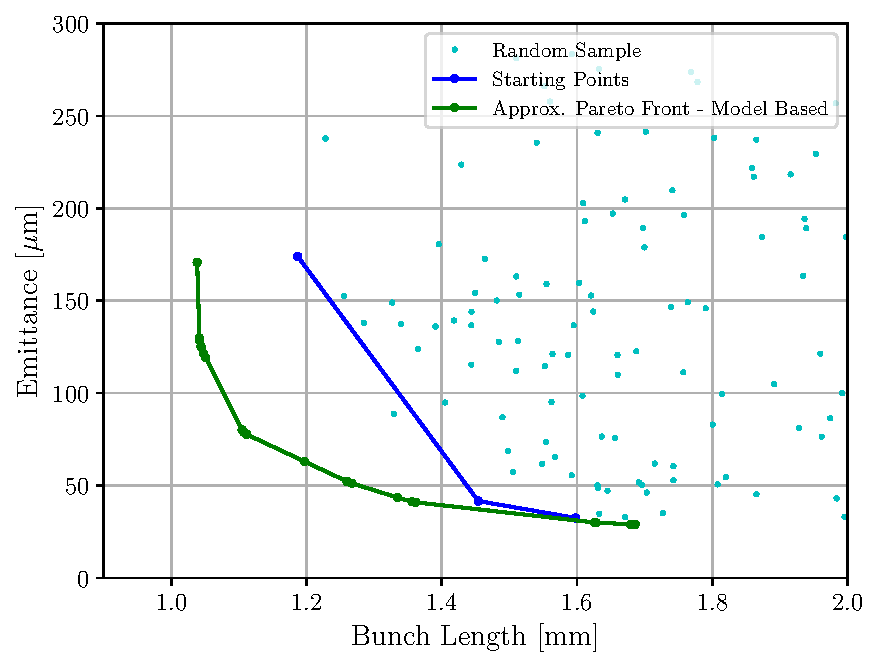
\includegraphics[width=0.5\textwidth]{pareto_emittance_vs_zrms}
	\caption{Pareto front for adjusted variable bounds. }
	\label{paretob}
\end{figure}



\section{Genetic Algorithms}
Explain what GA is....


GA's are very popular right now in accelerator physics,
and have been for several years \cite{bazarov, ga2, ga3}. 
Many have used GA's, and specifically NSGA-II \cite{nsgaii}, 
to tackle large multiobjective optimization problems. 
This is also the algorithm built into the simulation code 
OPAL \cite{opal}. 

To verify the method used in prior work, the fidelity of the model
was reduced and compared to a GA. 
\begin{figure}
	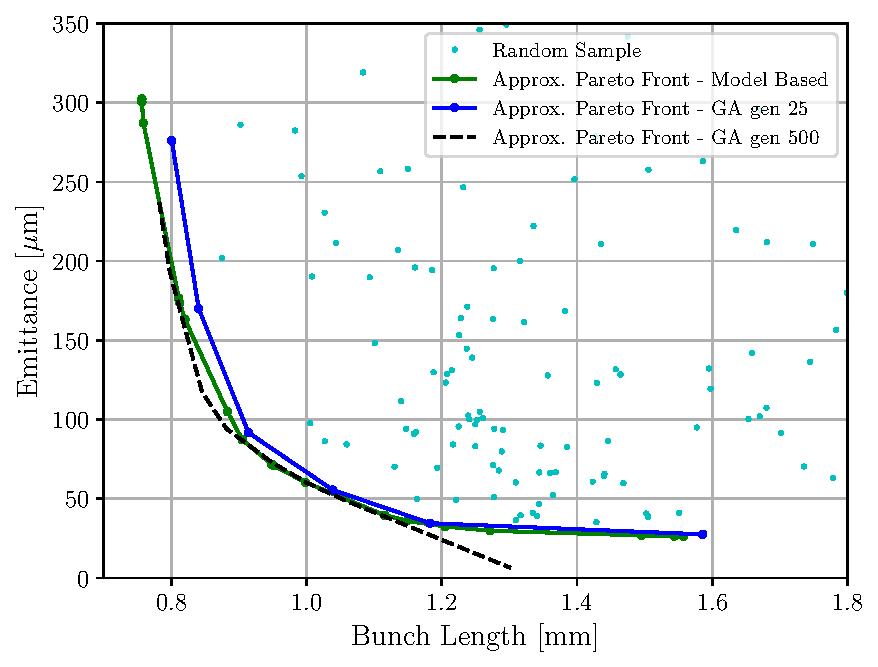
\includegraphics[width=0.5\textwidth]{model_vs_ga}
	\caption{Comparison of model based optimization and the GA implemented in OPAL. }
	\label{compare}
\end{figure}


\section{Results}
Simulations of the AWA beam line shown in Fig~\ref{beamline}
were performed in the PIC codes OPAL~\cite{opal}.
The gun, accelerating cavities, and solenoids were modeled with 2D
Poisson/Superfish~\cite{fish} files. All field maps were in the T7 format.
Input parameters for the simulations are shown in Table~\ref{simparam}.
Note that on crest refers to the phase of max energy gain.
In the case of the gun, a -~$20^{\circ}$ phase is measured 
w.r.t the phase of max energy gain. 
In other words, we ran $-20^{\circ}$ off crest.

\section{Future Work: Novel Methods}
In the following months, we plan to continue our work with
the Math and Computer Science (MCS) department at Argonne.
Using the library libensemble (\url{https://github.com/Libensemble/libensemble}), 
we will work to deploy methods being developed at ANL, such as APOSMM \cite{jeff}. 





\begin{table}[hbt]
	%   \vspace*{-.5\baselineskip}
	\centering
	\caption{Simulation Parameters}
	\begin{tabular}{lcc}
		\toprule
		\textbf{Parameter} & \textbf{Low Charge}  & \textbf{High Charge} \\
		\midrule
		Charge       & \SI{1}{nC}        & \SI{40}{nC}    \\ %[3pt]
		Gun Gradient & \SI{65}{MV/m}     & \SI{65}{MV/m}  \\ %[3pt]
		Gun Phase    & \SI{-20}{}$^{\circ}$ & \SI{-20}{}$^{\circ}$ \\		 
		$S_1$        & \SI{500}{A}		 & \SI{500}{A}	  \\
		$S_2$		 & \SI{}{A}   	 & \SI{185}{A}		 \\
		Linac Phases & On crest          & On crest       \\
		Laser FWHM   & \SI{1.5}{ps}      & \SI{1.5}{ps}   \\ %[3pt]
		Laser Radius & \SI{2}{mm}        & \SI{9}{mm}     \\
		\bottomrule
	\end{tabular}
	\label{simparam}
	%   \vspace*{-\baselineskip}
\end{table}


\begin{figure}[!htb]
	%   \vspace*{-.5\baselineskip}
	\centering
	%\includegraphics*[width=174pt]{JACpic_mc}
	\caption{Layout of papers.}
	\label{l2ea4-f1}
	%   \vspace*{-\baselineskip}
\end{figure}

\section{Conclusion}
Photoinjector optimization projects are ongoing at the AWA.
Two optimization methods have been used with success:
BOBYQA and NSGA-II. In the future, novel optimization 
methods developed at ANL will be tested. The first of 
which will be APOSMM. All optimization efforts are taking 
place to further operating conditions at the AWA and 
complete design work for upcoming experiments.


\section{acknowledgments}
We gratefully acknowledge the computing resources
provided on Bebop, a high-performance computing cluster
operated by the LCRC at Argonne National Laboratory.
This material is based upon work supported by the 
U.S. Department of Energy, Office of Science, under 
contract number DE-AC02-06CH11357 and grant number DE-SC0015479. 
Travel to IPAC'18 supported by the Division of Physics 
of the United States National Science Foundation 
Accelerator Science Program and the Division of 
Beam Physics of the American Physical Society.




\begin{thebibliography}{9}
\bibitem{eex}
G.~Ha \emph{et al.}, “Demonstration of Current Profile 
Shaping using Double Dog-Leg Emittance Exchange Beam 
Line at Argonne Wakefield Accelerator”
in \textit{Proc. IPAC’16}, 
Busan, South Korea, May 2016, 
paper TUOBB01.

\bibitem{pets}
J.~Shao \emph{et al.}, “Recent Progress towards Dielectric Short Pulse Two-Beam Acceleration”
in \textit{Proc. IPAC’18}, 
Vancouver, Canada, May 2018, 
paper TUYGBE3.

\bibitem{therm}
L.~Zheng \emph{et al.}, “Measurements of Thermal Emittance 
for Cesium Telluride Photocathodes in an L-Band RF Gun”
in \textit{Proc. IPAC’17}, 
Copenhagen, Denmark, May 2017, 
paper TUPAB074.

\bibitem{tba}
J.~Shao \emph{et al.}, “Recent Two-Beam 
Acceleration Activities at Argonne Wakefield Accelerator Facility”
in \textit{Proc. IPAC’17}, 
Copenhagen, Denmark, May 2017, 
paper WEPVA022.

\bibitem{nlopt}
M. Powell, “The BOBYQA algorithm for bound constrained
optimization without derivatives,” University of Cambridge,
U.K., Rep. NA2009/06, Oct. 2009.

\bibitem{denmark}
N.Neveu, J.Larson, J. G. Power, L. Spentzouris, 
“Photoinjector optimization using a derivative-free, model-based trust-region algorithm for the Argonne Wakefield Accelerator”
in \textit{Proc. IPAC’17}, 
Copenhagen, Denmark, May 2017, 
paper WEPVA022.

\bibitem{bazarov}
I. V. Bazarov, and C. K. Sinclair,
"Multivariate optimization of a high brightness dc gun photoinjector",
\emph{Phys. Rev. ST Accel. Beams}, vol. 8, p. 034202, March 2005. 



\bibitem{nsgaii}
K. Deb, A. Pratap, S. Agarwal and T. Meyarivan, 
"A Fast and Elitist Multiobjective Genetic Algorithm: NSGA-II," 
in IEEE Transactions on Evolutionary Computation, 
vol. 6, no. 2, pp. 182-197, Apr 2002.

\bibitem{opal}
A.~Adelmann \emph{et al.},
“The OPAL (Object Oriented Parallel Accelerator Library) framework,”
PSI, Zurich, Switzerland,
Rep. PSI-PR-08-02, 2008-2017.

\bibitem{fish}
\emph{Reference Manual for the POISSON/SUPERFISH Group of 
	Codes},  Los Alamos Accelerator Code Group,  
 Los Alamos, NM, USA, 
 Rep. LA-UR-87-126, Jan. 1987.
\end{thebibliography}



\end{document}
	
